\documentclass{article}
% Language setting
% Replace `english' with e.g. `spanish' to change the document language
\usepackage[english]{babel}
% Set page size and margins
% Replace `letterpaper' with `a4paper' for UK/EU standard size
\usepackage[letterpaper,top=2cm,bottom=2cm,left=3cm,right=3cm,marginparwidth=1.75cm]{geometry}
% Useful packages
\usepackage{multicol}
\usepackage{amsmath}
\usepackage{amssymb}
\usepackage{graphicx}
\usepackage[framemethod=tikz]{mdframed}
\usepackage{array}
\usepackage{blindtext}
%\usepackage[paperwidth=10cm]{geometry}
\usepackage{tkz-euclide}
%\usepackage{tikz}
\usetikzlibrary{
  circuits.logic,
  circuits.logic.US,
  positioning
}

\usepackage[colorlinks=true, allcolors=blue]{hyperref}
\newcommand{\myvec}[1]{\ensuremath{\begin{pmatrix}#1\end{pmatrix}}}
\providecommand{\norm}[1]{\left\lVert#1\right\rVert}
\let\vec\mathbf
\title{Circle Assignment}
\author{Anusha Jella}
\begin{document}
\maketitle
\newtheorem{theorem}{Theorem}[section]
\begin{multicols}{2}

\paragraph{\begin{flushleft}\textbf{Problem: }
\textbf{Draw a pair of tangents to a circle of radius 5 cm which are inclined to each other at an angle of 60$^{\circ}$.}
\end{flushleft}}
%\begin{figure}[h]
\centering
\includegraphics[scale=0.5]{circle_fig2.pdf}  
%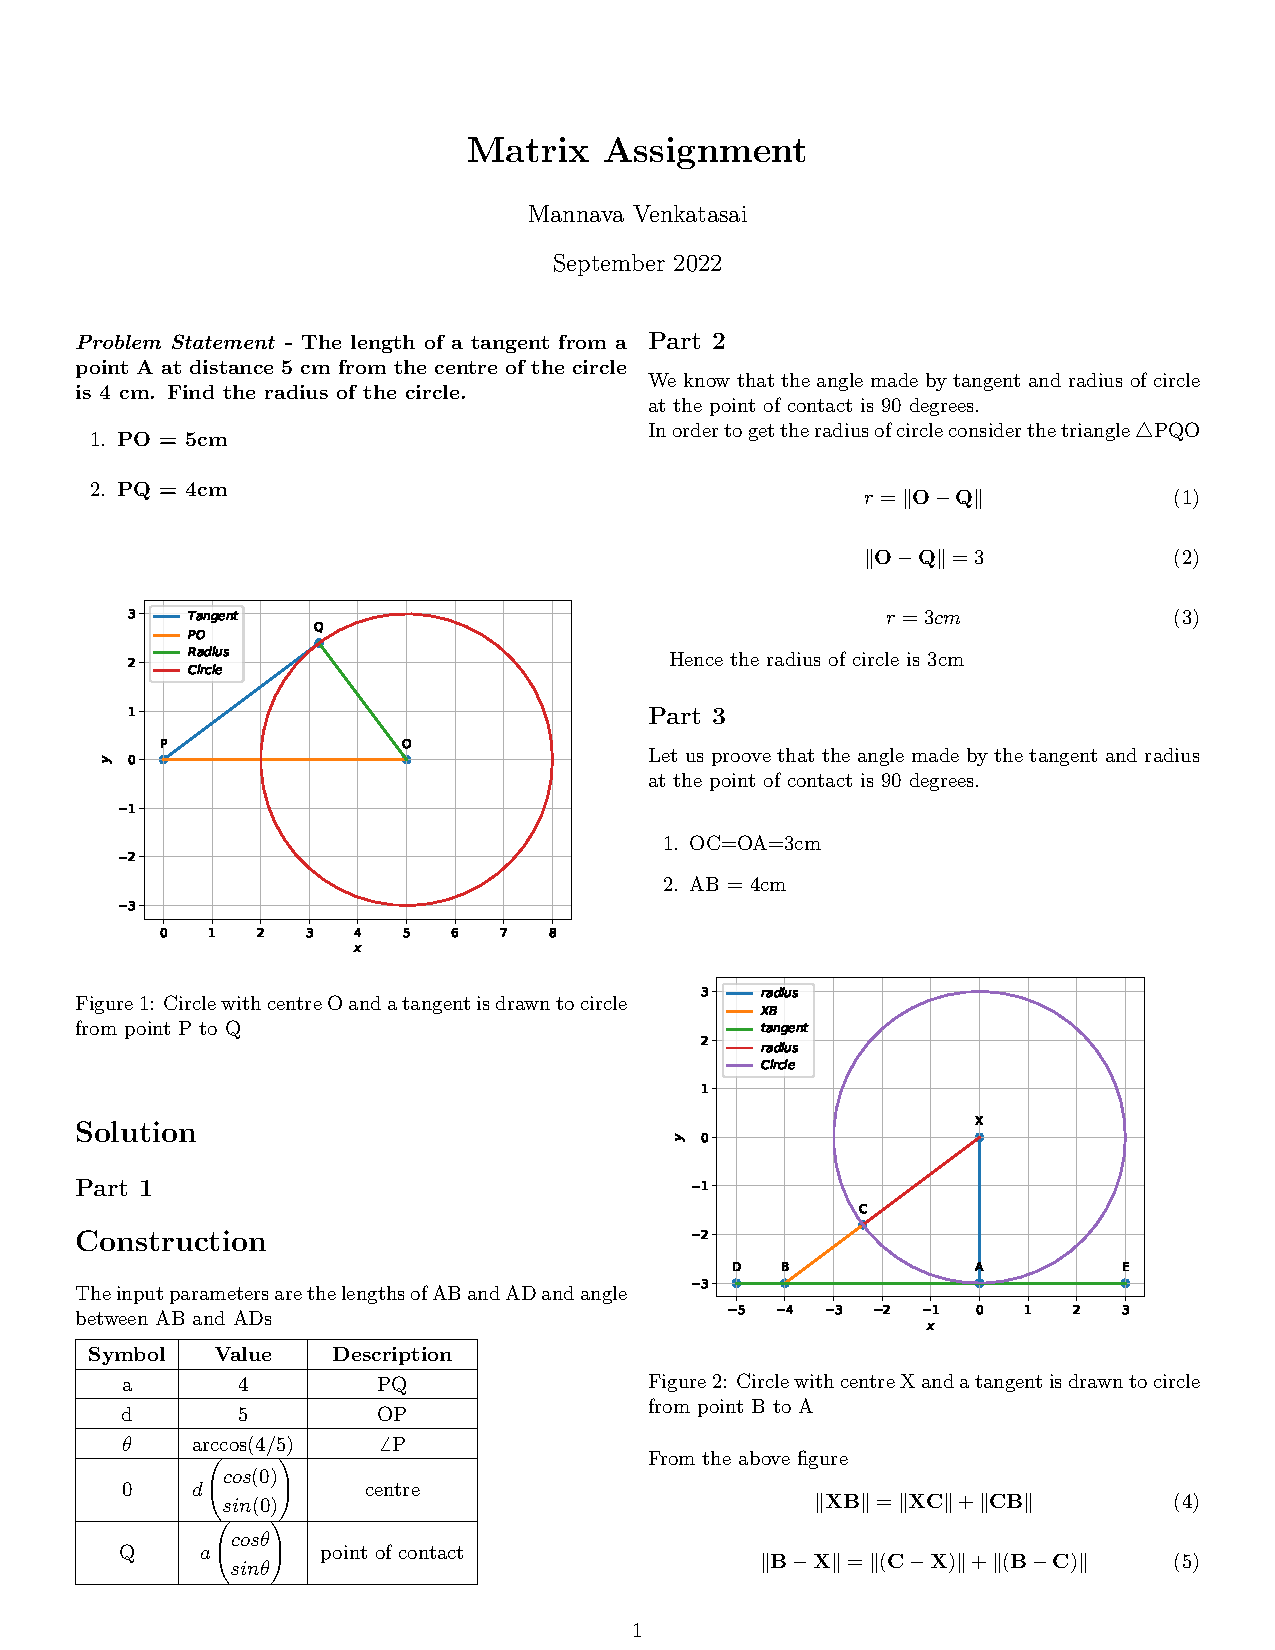
\includegraphics[width=\columnwidth]{circle1.pdf} 
\centering{Fig 1. Circle}
\label{fig:circle_1}
%\end{figure}

 \section*{Construction}
 \begin{flushleft}
 \textsc{solution:} The following python code is used for constructing circle with pair of tangents.
 \end{flushleft}
 \begin{mdframed}
   \url{https://github.com/AnushaJella/assignment_circle/blob/main/circle1.py}\\
\end{mdframed}
See Fig 1 for the input parameters in Table 1.\\
{\setlength\extrarowheight{2pt}
\begin{tabular}{|c|c|c|}
	\hline
	\textbf{Symbol}&\textbf{Value}&\textbf{Description}\\
	\hline
	O&$\begin{pmatrix}
	0\\0\\
	\end{pmatrix} $&Center $\vec{O}$\\
	\hline
	$\theta_{1}$&60$^{\circ}$& $\angle$$Q_1$P$Q_2$\\
	\hline
	r&5& radius of circle\\
	\hline
	
\end{tabular}
}\\
\centering {Table 1}\\
\hspace{-6cm}In $\Delta$Oqh 
\begin{align}
	\boldsymbol{h} = r\csc\frac{\theta}{2} e1
\end{align}
\section*{Solution}
\begin{flushleft}
The equation of  a conic with directrix $\vec{n}^{\top}\vec{x} = c$, eccentricity $e$ and focus $\vec{F}$ is given by 
\end{flushleft}
\begin{align}
    \vec{x}^{\top}\vec{V}\vec{x}+2\vec{u}^{\top}\vec{x}+f=0
\end{align}
\hspace{-2cm}for circle eccentricity e=0
then, 
\begin{align}
	\vec{V}
	=\vec{I},
\vec{u} = \myvec{0\\0},  f = -r^2.
	\label{eq:matrix-10-13-param}
\end{align}
\hspace{-2.5cm}Point q on conic is given by
\begin{align*}
q=\vec{V}^{-1}(k_i\vec{n}-\vec{u}^T)^T \\
\hspace{-6cm}where,\\
k_i=\pm \sqrt{\frac{f_0}{\vec{n}^T\vec{V}^{-1}\vec{n}}}\\
f_0=f+\vec{u}^T\vec{V}^{-1}\vec{u}\\
n=P\myvec{\sqrt{\lambda_1}\\\pm \sqrt{\lambda_2}}
\end{align*}
\hspace{-2cm}$\vec{P}$,$\lambda_{1,2}$ are eigen parameters of 
\begin{align*}
\sum=(\vec{V}\vec{h}+\vec{u})(\vec{V}\vec{h}+\vec{u})^T-\vec{V}(\vec{h}^T\vec{V}\vec{h}+2\vec{u}^Th+f)
\end{align*}
\end{multicols}{2}
\end{document}
